% !TEX root = ../main.tex
%--- Slide 10: un band noise che non si vede (circa 50 s) --------------------------------
% Figura: Figure/P11_logA_BN_due_pannelli.pdf (notebook 26): posterior di log10 A_BN,
% dati reali (blu) vs simulazione (viola) iniettata a -12.5 e a -12, modello a 8 parametri.
\begin{frame}{Un band noise che non si vede}
  \small
  \textcolor{simdue}{Simulazioni} analizzate con il band noise nel modello (8 parametri)
  \begin{itemize}\setlength{\itemsep}{1pt}
    \item Il band noise resta non rivelato fino a $-12.5$ ($\log_{10}A_{\rm BN} < -12.36$ al 95\%)
          e viene rivelato solo a $-12$, perché i TOA di LOFAR hanno grandi incertezze
    \item \reali{Dati reali}: $\log_{10}A_{\rm BN} < -12.21$ (95\%), simile alla simulazione con $-12.5$
    \item Un band noise non rivelato può indurre un bias nel DM
    \item \textbf{Non può essere esclusa la presenza di un band noise nei dati reali}
  \end{itemize}
  \vspace{1mm}
  \centering
  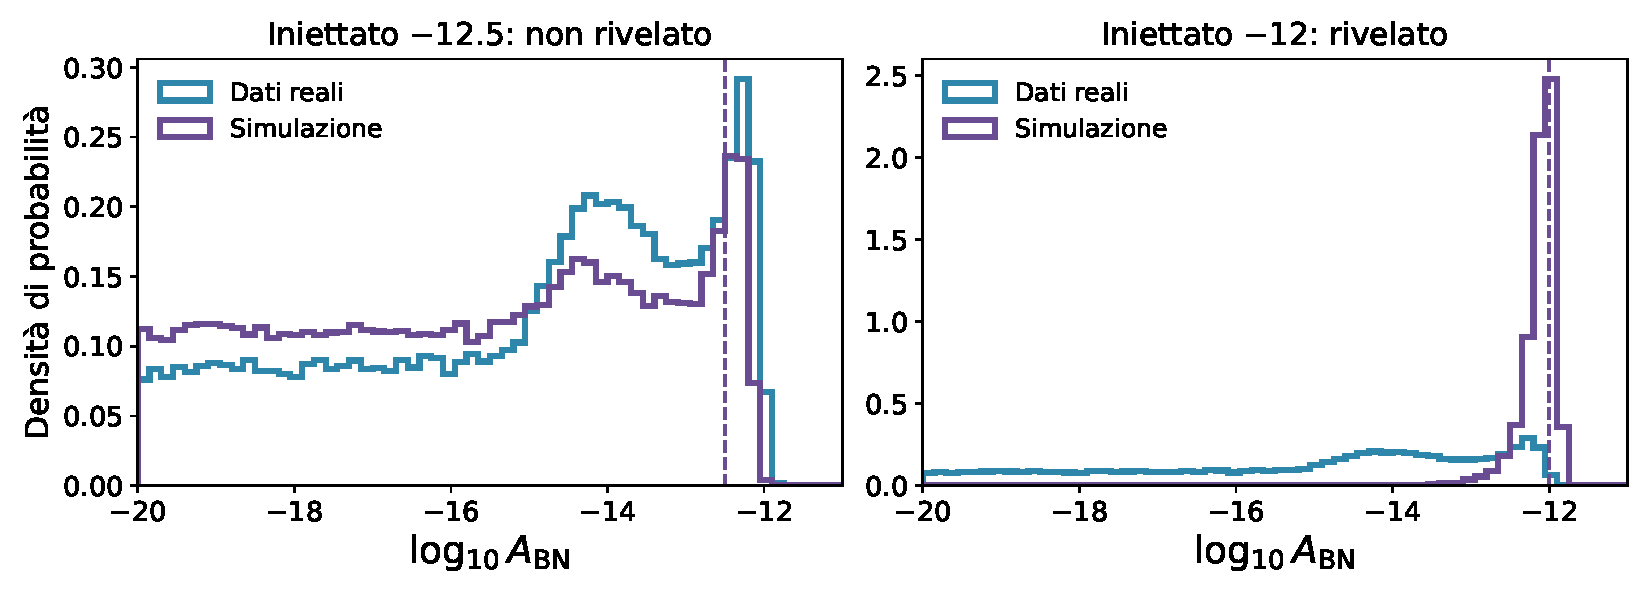
\includegraphics[width=0.80\textwidth]{Figure/P11_logA_BN_due_pannelli.pdf}
\end{frame}
